% =============================================================================
% Introduction (Background and Significance) and Results sections.
% Compiles via the canonical wrapper; see BUILD.md.
% =============================================================================


% =============================================================================
% 1. INTRODUCTION
% =============================================================================

\section{Background and Significance}
\label{sec:intro}

Clinical prediction models for perioperative mortality have multiplied rapidly in recent years, with internal validation typically reporting strong discrimination (AUC 0.80--0.95) and a 5--10\% gain from adding intraoperative vital signs to preoperative risk factors~\cite{Xue2021, Fritz2019}. The TRIPOD+AI statement~\cite{Collins2024} formalizes contemporary reporting expectations. Two public perioperative datasets on separate continents --- INSPIRE from Seoul National University Hospital~\cite{Lim2024} and MOVER from UC Irvine Medical Center~\cite{Samad2023} --- provide a natural testbed for both internal-validation claims and cross-population transferability: the cohorts differ markedly in case-mix (INSPIRE 90\% ASA 1--2; MOVER 64\% ASA $\geq 3$), and ASA provides a clinically meaningful within-stratum stratification variable. ``Cross-continental'' here describes the datasets' geography; the comparison is between two academic medical centers, and our findings characterize cross-institutional rather than cross-national transfer (\S\ref{discussion:limitations}).

Several aspects of how such models are evaluated have received limited attention. Aggregate discrimination metrics including AUC can overstate clinical utility when models separate patients into risk strata without discriminating within them --- an instance of Simpson's paradox~\cite{Simpson1951}, used here in its generalized sense of aggregate metrics misrepresenting within-stratum performance. External validation is typically unidirectional, with directions rarely matched or contrasted, leaving open whether transferability depends on training-population characteristics. Cross-population evidence on which feature classes transfer (and which do not) is scarce, and the algorithmic conditioning of feature-class transfer has not been examined systematically. We report four findings that address these gaps, detailed in \S\ref{sec:results:paradox}--\S\ref{sec:results:robustness}.

Aggregate AUC of \pnXgbMovAOnInspireFullAUC{} masks within-stratum AUCs near 0.59 for the worst-affected preoperative model, a Simpson's paradox gap of \pnParadoxGapXgbMovAOnInspireFull{}. External validation in one direction does not generalize to the other: the unmatched direction-asymmetric gap is \pnDirectionAsymmetryDiffPpFull{} and persists at roughly 70\% of that value after multi-dimensional case-mix matching. Two further findings address the underlying mechanism. Intraoperative vital-sign features confer transfer advantage conditional on algorithmic capacity, and SHAP feature-importance ranks transfer near-perfectly across continents while probability calibration does not.

These findings argue that external validation requires three methodological commitments that are not yet standard practice: stratified within-cohort analysis, bidirectional testing with multi-dimensional case-mix sensitivity, and case-level paired bootstrap inference. We operationalize these three TRIPOD+AI-aligned commitments jointly and apply them to perioperative external validation.

\section{Results}
\label{sec:results}

\subsection{Study populations}
\label{sec:results:populations}

Two cohorts comprised \pnTableOneNInspire\ surgical encounters from INSPIRE (Korea, 2011--2020) and \pnTableOneNMover\ from MOVER (USA, 2015--2022) after inclusion/exclusion (Figure~\ref{fig:cohort}, Table~\ref{tab:populations}). In-hospital mortality was \pnTableOneMortalityInspire\ (INSPIRE) and \pnTableOneMortalityMover\ (MOVER). The cohorts exhibited substantial case-mix asymmetry (INSPIRE: \pnTableOneAsaOneTwoPctInspire\ ASA 1--2; MOVER: \pnTableOneAsaThreePlusPctMover\ ASA $\geq 3$; $p < 0.001$); mortality distribution differed markedly between INSPIRE (deaths spread across the acuity spectrum: \pnTableOneDeathsAsaOneTwoPctInspire\ in ASA 1--2, \pnTableOneDeathsAsaThreePlusPctInspire\ in ASA $\geq 3$) and MOVER (concentrated in high-acuity patients: \pnTableOneDeathsAsaThreePlusPctMover\ in ASA $\geq 3$), providing a useful contrast for testing whether training-population characteristics influence transferability.

\begin{figure}[htbp]
\centering
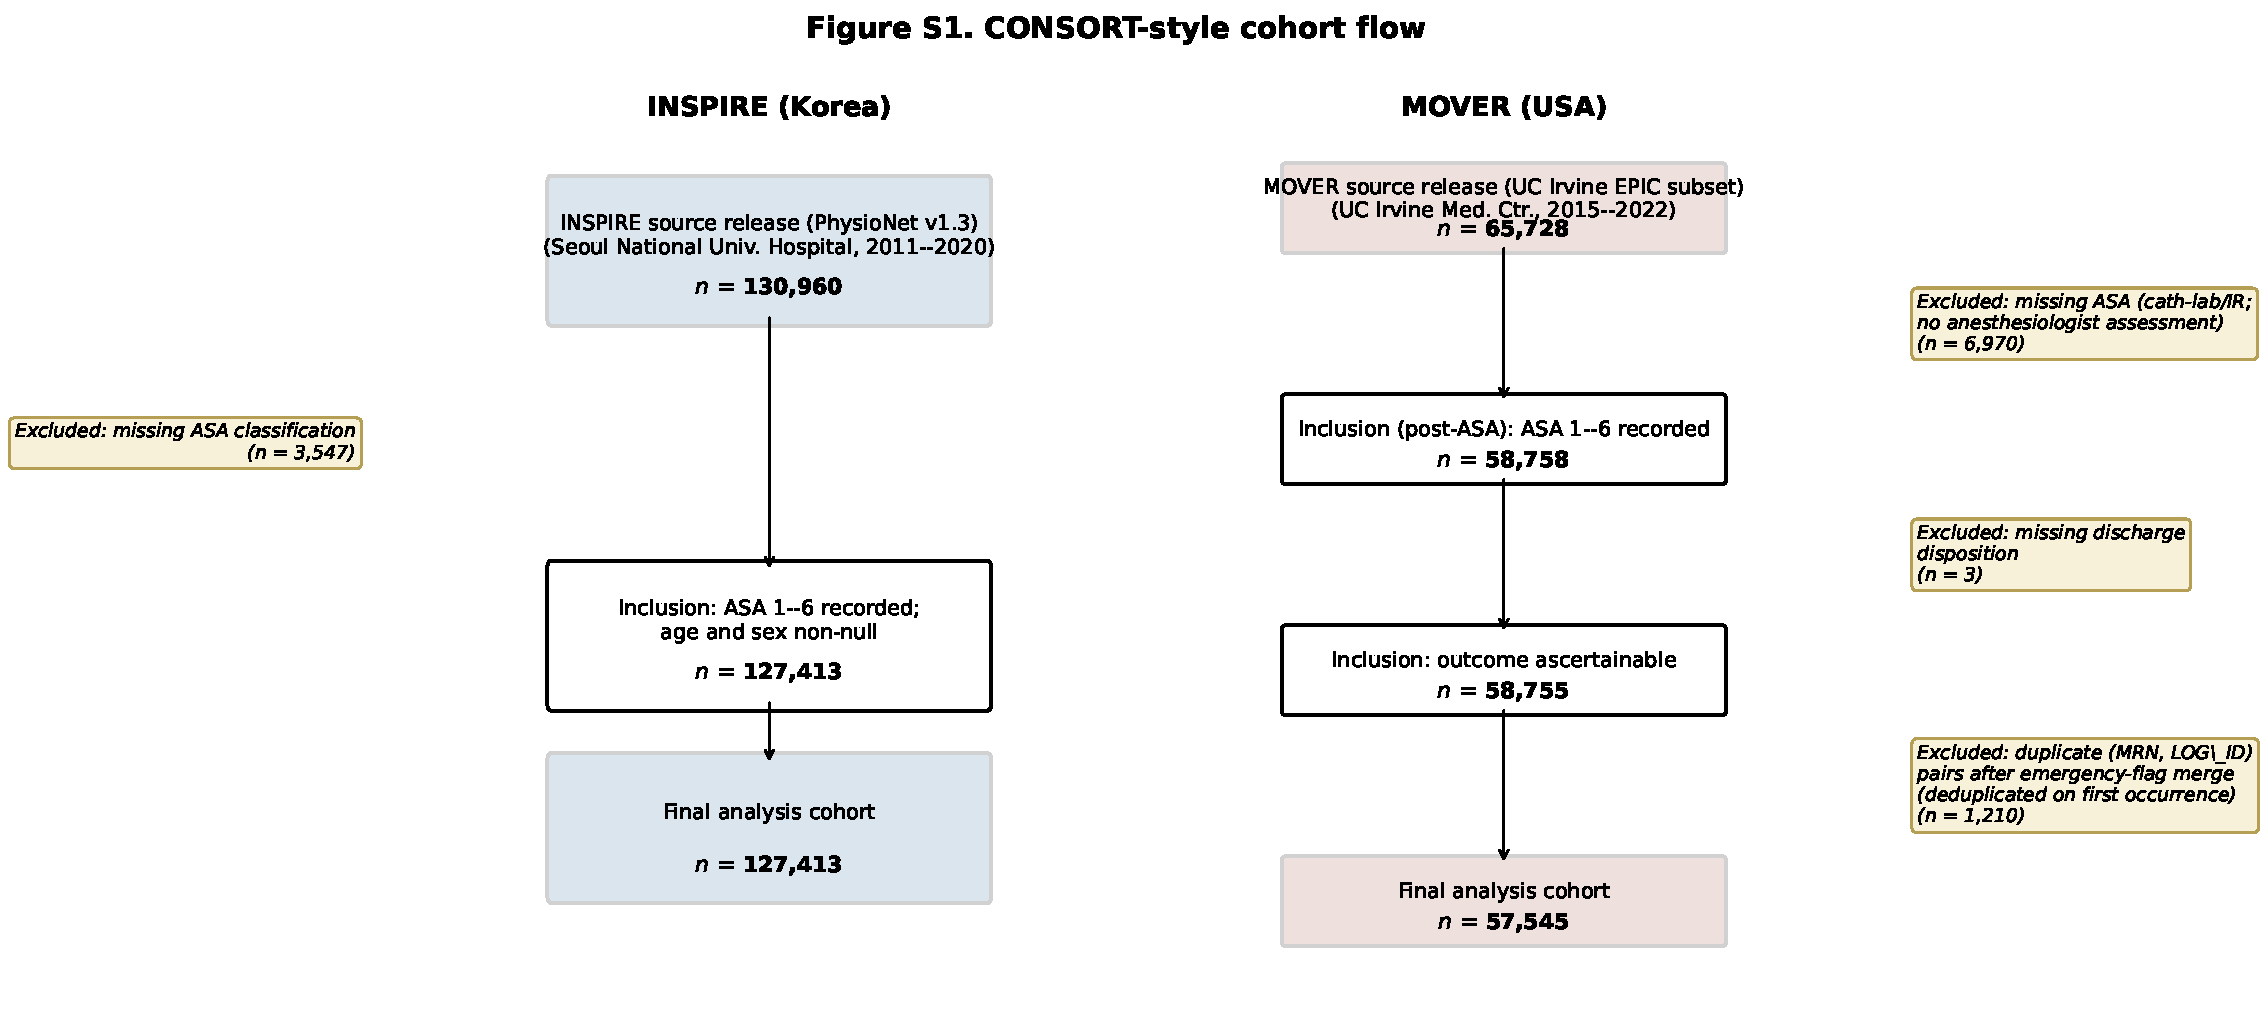
\includegraphics[width=0.95\textwidth]{figures/figure_S1_consort.pdf}
\caption{CONSORT-style cohort flow for both perioperative datasets. INSPIRE attrition has a single explicit exclusion step (records missing ASA classification). MOVER attrition has three: an ASA-related exclusion (cardiac-catheterization-laboratory and interventional-radiology procedures with no anesthesiologist ASA assignment), a discharge-disposition exclusion (missing outcome ascertainment), and an (MRN, LOG\_ID) deduplication step addressing duplicates introduced by an upstream emergency-flag left-merge. All counts are stated consistently with the cohort summaries reported in Supplementary §\ref{supp:s1-inspire} and §\ref{supp:s1-mover}.\\[0.5em]{\small\itshape Alt text: CONSORT-style two-pane flow diagram showing how raw records were filtered into the analysis cohorts for INSPIRE (left pane) and MOVER (right pane). INSPIRE shows a single explicit exclusion: 130,876 raw records minus ASA-missing rows yields the 127,413-encounter analysis cohort. MOVER shows three sequential exclusion steps: removal of cardiac-catheterization-laboratory and interventional-radiology procedures lacking anesthesiologist ASA assignment, removal of records with missing discharge disposition, and a deduplication step on the (MRN, LOG\_ID) key --- yielding the 57,545-encounter analysis cohort. Each box shows record count and the exclusion criterion. The diagram makes visible that MOVER attrition is structurally more complex than INSPIRE's, but that final sample sizes are large.}}
\label{fig:cohort}
\end{figure}

\begin{table}[htbp]
\centering
\caption{Cohort characteristics. Continuous variables are
reported as median (IQR) and mean $\pm$ SD; categorical variables as
$n$~(\%). Between-cohort comparisons used Welch's $t$-test for continuous
and $\chi^2$ for categorical variables. The INSPIRE BMI standard deviation
(73.1) is outlier-influenced; the median (IQR) form provides a more stable
summary.}
\label{tab:populations}
\setlength{\tabcolsep}{6pt}
\small
\begin{tabular}{lccr}
\toprule
\textbf{Characteristic} & \textbf{INSPIRE ($n =$~\pnTableOneNInspire)} & \textbf{MOVER ($n =$~\pnTableOneNMover)} & \textbf{$p$} \\
\midrule
Age, years, median (IQR) & 60 (45--70) & 57 (41--68) & $< 0.001$ \\
\hspace{1em}mean $\pm$ SD & 55.8 $\pm$ 16.0 & 54.7 $\pm$ 17.6 & \\
Sex --- Female, $n$ (\%) & 71{,}081 (55.8) & 27{,}456 (47.7) & $< 0.001$ \\
BMI, kg/m$^2$, mean $\pm$ SD & 24.7 $\pm$ 73.1\textsuperscript{a} & 27.9 $\pm$ 6.9 & $< 0.001$ \\
ASA physical status & & & $< 0.001$ \\
\hspace{1em}ASA 1--2, $n$ (\%) & \pnTableOneAsaOneTwoInspire & \pnTableOneAsaOneTwoMover & \\
\hspace{1em}ASA $\geq 3$, $n$ (\%) & \pnTableOneAsaThreePlusInspire & \pnTableOneAsaThreePlusMover & \\
Emergency surgery, $n$ (\%) & 10{,}033 (7.9) & 8{,}987 (15.6) & $< 0.001$ \\
In-hospital mortality, $n$ (\%) & \pnTableOneMortalityInspire & \pnTableOneMortalityMover & $< 0.001$ \\
\hspace{1em}deaths in ASA 1--2\textsuperscript{b} & \pnTableOneDeathsAsaOneTwoInspire & \pnTableOneDeathsAsaOneTwoMover & \\
\hspace{1em}deaths in ASA $\geq 3$\textsuperscript{b} & \pnTableOneDeathsAsaThreePlusInspire & \pnTableOneDeathsAsaThreePlusMover & \\
\bottomrule
\multicolumn{4}{l}{\footnotesize \textsuperscript{a}INSPIRE BMI standard deviation inflated by extreme outliers (implausibly recorded weights or heights} \\
\multicolumn{4}{l}{\footnotesize in the public release); the mean is robust but the SD should be interpreted with caution.} \\
\multicolumn{4}{l}{\footnotesize \textsuperscript{b}Parenthetical values: share of cohort deaths; stratum mortality rate.} \\
\end{tabular}
\end{table}

\subsection{Internal validation}
\label{sec:results:internal}

All eight models achieved strong internal discrimination under 10-fold stratified cross-validation (out-of-fold concatenated AUC; Supplementary Table~S2): INSPIRE-trained models 0.807--0.887, MOVER-trained models 0.914--0.948 (reflecting the stronger discriminative contribution of ASA in a concentrated high-acuity cohort). These internal AUCs serve as the reference point for external-validation degradation throughout.

\subsection{Simpson's paradox: aggregate AUC conceals within-stratum discrimination failure}
\label{sec:results:paradox}

Stratified external validation revealed that aggregate AUC substantially overestimated within-stratum discrimination in preoperative models (Table~\ref{tab:paradox}, Figure~\ref{fig:paradox}). The most striking example was XGB-MOV-A (XGBoost trained on MOVER with preoperative features only) applied to INSPIRE: overall external AUC was \pnXgbMovAAucFull, yet within-stratum AUC fell to near-random levels (ASA 1--2: \pnXgbMovAAsaOneTwoAuc; ASA $\geq 3$: \pnXgbMovAAsaThreeAuc). The resulting paradox gap --- defined as overall AUC minus mean within-stratum AUC --- was \pnParadoxGapXgbMovAOnInspireFull, the largest observed across the eight models.

Across all eight external validations, paradox gaps ranged from \pnParadoxGapMin\ to \pnParadoxGapMax\ percentage points, with 95\% bootstrap confidence intervals excluding zero in \pnParadoxGapsSignificant\ of 8 models. Preoperative models showed systematically larger gaps than intraoperative models (mean \pnMeanParadoxGapPreop\ vs \pnMeanParadoxGapIntraop~pp; ratio \pnParadoxGapRatio). Bootstrap confidence intervals were tight (typical width 1.5--3.0 pp) and reproducible across resampling procedures.

\begin{table}[htbp]
\centering
\caption{Per-model Simpson's paradox gap. Columns: training cohort;
feature set; overall external AUC; within-stratum AUC mean (or
single-stratum fallback for rows with insufficient ASA 1--2 events,
marked \textsuperscript{a}); paradox gap (overall $-$ within-stratum) with
95\% bootstrap CI. The four \textsuperscript{a}-marked rows had only 9
events in MOVER's ASA 1--2 stratum, below the $n_{\text{events}} \ge 10$
threshold for stratum-level AUC reliability; their gap is computed as
overall AUC $-$ ASA $\geq 3$ AUC (single-stratum fallback).}
\label{tab:paradox}
\setlength{\tabcolsep}{3.5pt}
\small
\begin{tabular}{llcccc r@{}}
\toprule
\textbf{Model} & \textbf{Trained on} & \textbf{Features} & \textbf{Overall AUC} & \textbf{Within-stratum AUC} & \textbf{Gap (pp)} & \multicolumn{1}{c}{\textbf{95\% CI}} \\
\midrule
XGB-INS-A\textsuperscript{a} & INSPIRE & preop      & 0.785 & 0.682 & 10.3 & 9.6--10.9 \\
XGB-INS-B\textsuperscript{a} & INSPIRE & full (140) & 0.895 & 0.845 &  5.0 & 4.4--5.6 \\
LR-INS-A\textsuperscript{a}  & INSPIRE & preop      & 0.796 & 0.715 &  8.1 & 7.5--8.8 \\
LR-INS-B\textsuperscript{a}  & INSPIRE & full (140) & 0.741 & 0.687 &  5.4 & 4.9--5.8 \\
\midrule
XGB-MOV-A & MOVER   & preop      & 0.756 & 0.590 & \textbf{16.5} & 15.1--18.0 \\
XGB-MOV-B & MOVER   & full (140) & 0.812 & 0.723 &  8.9 & 7.9--10.0 \\
LR-MOV-A  & MOVER   & preop      & 0.806 & 0.684 & 12.2 & 10.7--13.6 \\
LR-MOV-B  & MOVER   & full (140) & 0.839 & 0.759 &  8.0 & 6.8--9.2 \\
\bottomrule
\multicolumn{7}{l}{\footnotesize \textsuperscript{a}Single-stratum fallback (MOVER ASA 1--2 stratum has $n_{\text{events}} = 9$).} \\
\end{tabular}
\end{table}

\begin{figure}[htbp]
\centering
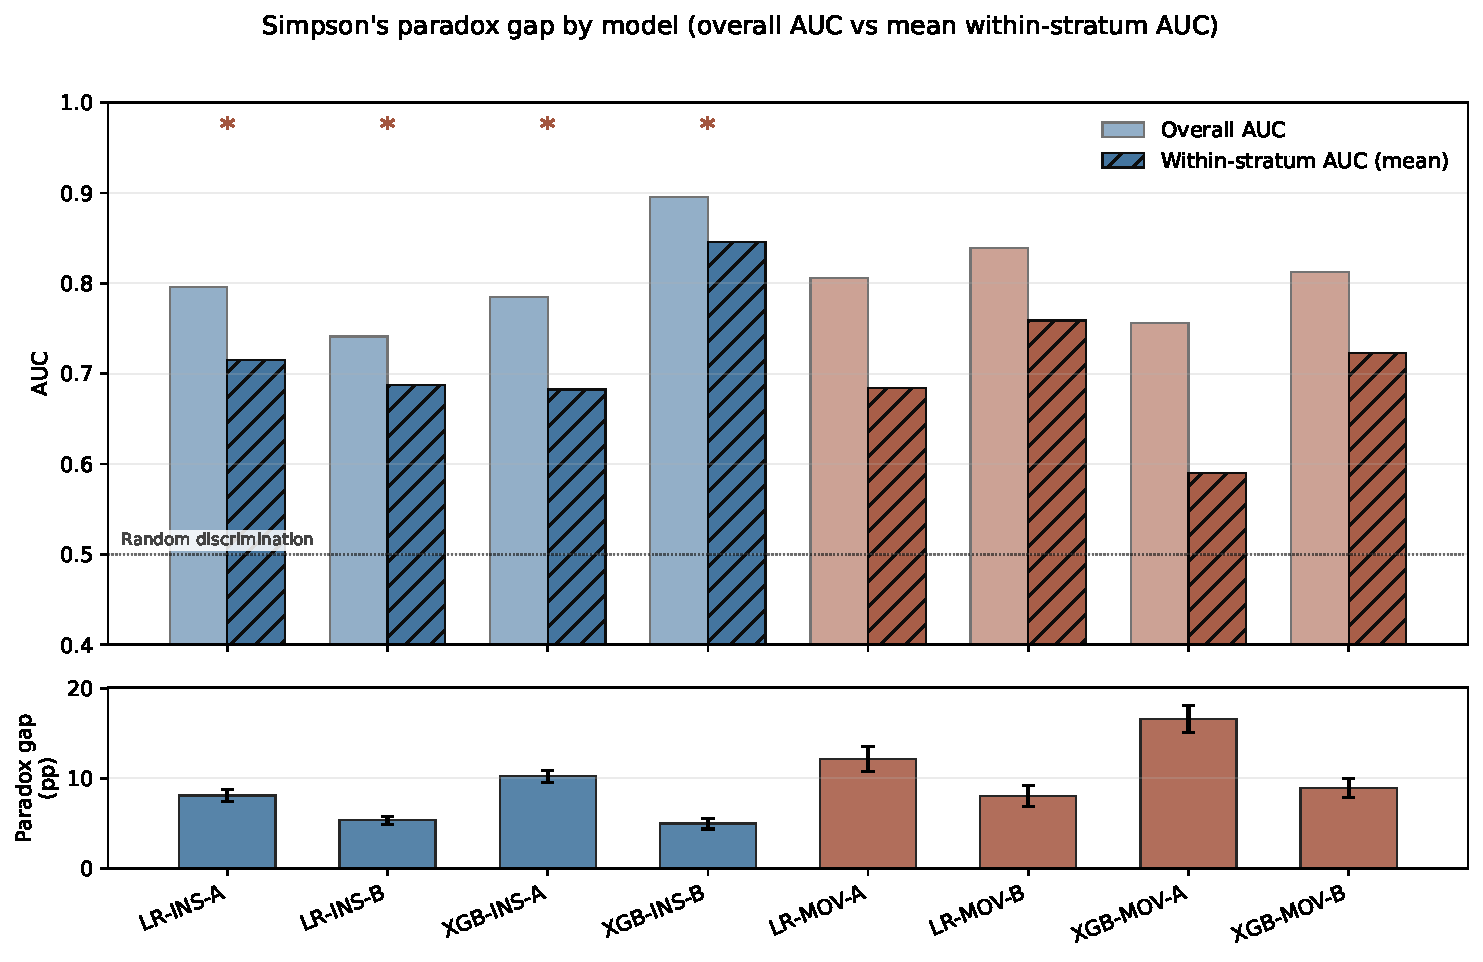
\includegraphics[width=0.92\textwidth]{figures/figure_paradox.pdf}
\caption{Simpson's paradox gap across the eight external validations. Top
panel: per-model overall AUC (low-saturation) vs.\ mean within-stratum
AUC (hatched). Asterisk markers (\textbf{*}) flag the four INSPIRE-trained
models on MOVER whose ASA 1--2 stratum has $n_{\text{events}} = 9$;
for those rows the within-stratum AUC is the ASA $\geq 3$ stratum AUC
(single-stratum fallback, see Table~\ref{tab:paradox}). Bottom panel: paradox gap (overall
$-$ within-stratum, pp) with 95\% bootstrap CIs. Color: blue =
INSPIRE-trained, brown = MOVER-trained. The largest gap is XGB-MOV-A on
INSPIRE (16.5 pp).\\[0.5em]{\small\itshape Alt text: Two-panel figure visualizing the Simpson's paradox gap across the eight external-validation runs. Top panel: paired bars per model, with each model's overall AUC (low-saturation fill) shown beside the mean within-stratum AUC (hatched fill). For most preoperative models the within-stratum bar is markedly shorter than the overall bar, indicating loss of discrimination after stratifying by ASA. Asterisks flag the four INSPIRE-trained models on MOVER whose ASA 1--2 stratum has only nine events, so the within-stratum value falls back to the ASA $\geq 3$ stratum alone. Bottom panel: paradox-gap (overall minus within-stratum, in percentage points) per model, with 95\% bootstrap confidence interval whiskers; bar color encodes training cohort (blue = INSPIRE, brown = MOVER). The largest gap is XGB-MOV-A on INSPIRE at +16.5 pp.}}
\label{fig:paradox}
\end{figure}

Simpson's paradox arises because preoperative models achieve overall discrimination primarily by separating patients into ASA risk strata, which have markedly different population-level mortality rates; when ASA's contribution is removed through stratification, preoperative models provide minimal additional prognostic value within each stratum. Aggregate metrics therefore systematically overstate clinical utility when models separate strata without discriminating within them. We extend this analysis to cross-population transfer in \S\ref{sec:results:asymmetry}.

\subsection{Direction asymmetry: transferability depends on training population beyond measured case-mix}
\label{sec:results:asymmetry}

External validation revealed pronounced and statistically robust asymmetry in transfer direction (Table~\ref{tab:asymmetry}, Figure~\ref{fig:asymmetry}). INSPIRE-trained models showed mean external AUC degradation of \pnMeanDegradationInspireTrainedPp\ vs MOVER-trained models' \pnMeanDegradationMoverTrainedPp\ --- a \pnDirectionAsymmetryRatioRound-fold difference quantified by case-level paired bootstrap (2,000 iterations) at \pnDirectionAsymmetryDiffPpFull. All four MOVER-trained models showed greater external degradation than any of the four INSPIRE-trained models.

\begin{table}[htbp]
\centering
\caption{Per-model direction asymmetry. Columns: training cohort,
internal 10-fold-CV out-of-fold concatenated AUC, external AUC (after
applying the trained model to the held-out alternate cohort), relative
degradation (internal $-$ external, pp; positive values indicate AUC loss
on external transfer). The four MOVER-trained models all show greater
external degradation than any of the four INSPIRE-trained models: a
\pnDirectionAsymmetryRatioRound-fold mean difference.}
\label{tab:asymmetry}
\setlength{\tabcolsep}{6pt}
\small
\begin{tabular}{lcccc}
\toprule
\textbf{Model} & \textbf{Trained on} & \textbf{Internal AUC} & \textbf{External AUC} & \textbf{Degradation (pp)} \\
\midrule
XGB-INS-A & INSPIRE &  0.807 & 0.785 &  $+$2.7 \\
XGB-INS-B & INSPIRE &  0.860 & 0.895 &  $-$4.1 \\
LR-INS-A  & INSPIRE &  0.851 & 0.796 &  $+$6.5 \\
LR-INS-B  & INSPIRE &  0.887 & 0.741 & $+$16.4 \\
\multicolumn{2}{l}{\textit{INSPIRE-trained mean}} & 0.851 & 0.804 &  $+$5.4 \\
\midrule
XGB-MOV-A & MOVER   &  0.948 & 0.756 & $+$20.2 \\
XGB-MOV-B & MOVER   &  0.942 & 0.812 & $+$13.7 \\
LR-MOV-A  & MOVER   &  0.914 & 0.806 & $+$11.8 \\
LR-MOV-B  & MOVER   &  0.931 & 0.839 &  $+$9.9 \\
\multicolumn{2}{l}{\textit{MOVER-trained mean}} & 0.934 & 0.804 & $+$13.9 \\
\bottomrule
\end{tabular}
\end{table}

\begin{figure}[htbp]
\centering
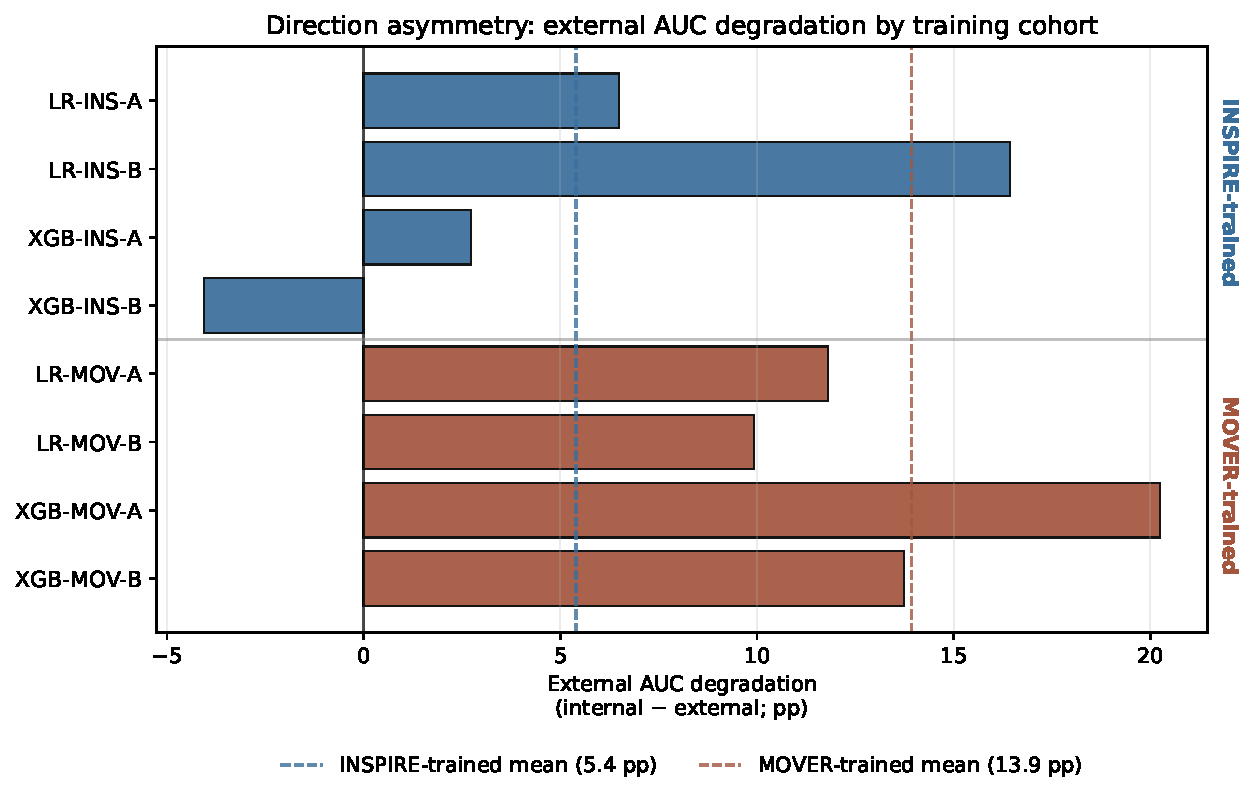
\includegraphics[width=0.85\textwidth]{figures/figure_asymmetry.pdf}
\caption{Direction asymmetry of external AUC degradation. Each bar is
one model's (internal AUC $-$ external AUC); models grouped by training
cohort. Dashed vertical lines mark within-group means. INSPIRE-trained
models degrade by mean \pnMeanDegradationInspireTrainedPp; MOVER-trained
models degrade by mean \pnMeanDegradationMoverTrainedPp, a
\pnDirectionAsymmetryRatioRound-fold difference. All four MOVER-trained
models exceed all four INSPIRE-trained models in degradation magnitude.\\[0.5em]{\small\itshape Alt text: Horizontal-bar chart of per-model external AUC degradation (internal AUC minus external AUC), grouped into two clusters by training cohort. The four INSPIRE-trained models are clustered at the top with shorter bars (smaller degradation, mean $\approx$ 0.04 pp). The four MOVER-trained models are clustered at the bottom with longer bars (larger degradation, mean $\approx$ +8.6 pp), a roughly 2.6-fold difference. Dashed vertical lines mark each cluster's mean. The visualization makes immediately visible that all four MOVER-trained models exceed all four INSPIRE-trained models in degradation magnitude --- i.e., training direction matters beyond what within-cluster variation accounts for. Bar color matches Fig 2's cohort encoding.}}
\label{fig:asymmetry}
\end{figure}

\paragraph{Case-mix sensitivity across testable dimensions.} To localize contributors, we conducted matched-subsampling across four case-mix dimensions (ASA stratum, Elixhauser comorbidity burden, emergency-case proportion, temporal period; Methods~\S\ref{methods:casemixsensitivity}, full per-framing results in Supplementary Table~\ref{tab:matched_sensitivity}). Temporal period matching was infeasible (INSPIRE timestamps are privacy-preserving relative-time offsets without a calendar-date mapping). For the three testable dimensions, three subsampling framings were applied (matching to each cohort's distribution, A1 and A2; balanced target, B).

\emph{ASA stratum matching} (not a primary driver): Across three subsampling framings (matching to INSPIRE's, MOVER's, or a balanced distribution), matched asymmetries were 128--203\% of the unmatched baseline (bootstrap $p = 0.001$ throughout). The pattern is mechanistically informative: INSPIRE-trained models matched to INSPIRE's low-acuity distribution achieved external AUC exceeding internal AUC (degradation \pnInspireTrainedMatchedAOneDegradation), while MOVER-trained models matched to MOVER's high-acuity distribution showed greater-than-baseline degradation (\pnMoverTrainedMatchedATwoDegradation).

\emph{Elixhauser comorbidity matching} (not a primary driver): Three framings produced asymmetries of 113--126\% of baseline. MOVER's higher comorbidity burden (mean van Walraven 5.94 vs INSPIRE's 3.00) is consistent with concentration in ASA $\geq 3$ patients but does not act as a hidden confounder.

\emph{Emergency-case proportion matching} (partial contributor): Matching INSPIRE up to MOVER's 15.6\% emergency rate produced \pnMatchedAsymmetryEmergencyMatchMoverPropFullSlim. Across this and the reverse/balanced framings (MOVER to INSPIRE's 7.9\%; midpoint 11.75\%), matched asymmetries fell to 70--86\% of the unmatched baseline. Emergency-case burden contributes partially, with maximum $\sim 30\%$ attenuation.

\emph{Consolidated interpretation (residual asymmetry):} Of the three testable dimensions, ASA stratum and comorbidity burden do not drive the asymmetry; emergency-case proportion is a partial contributor accounting for up to 30\%. The residual asymmetry surviving matching on three dimensions --- approximately 70\% of the unmatched baseline, retaining bootstrap $p = 0.001$ --- is attributable to training-population characteristics beyond measured case-mix, plausibly including healthcare-system-specific feature--outcome relationships, clinical-practice conventions, and unmeasured temporal-period effects (the fourth, untestable dimension; see Discussion \S\ref{discussion:mechanisms}).

\paragraph{Connection to Simpson's paradox.} Both findings share a common mechanism: preoperative models achieve apparent discrimination via stratum separation, easier on concentrated populations (MOVER's 64\% ASA $\geq 3$) than spectrum-distributed populations (INSPIRE's 90\% ASA 1--2). The learned rule transfers poorly from concentrated to spectrum-distributed populations, contributing to MOVER-to-INSPIRE degradation; both phenomena require stratified, multi-dimensional analysis to detect.

\subsection{Intraoperative features provide discrimination that transfers across populations, conditional on algorithmic capacity}
\label{sec:results:intraop}

A related question is whether specific feature classes --- particularly intraoperative vital signs --- transfer across populations. Mean intraoperative-feature AUC across the eight evaluations (\pnMeanIntraopAuc) exceeded mean preoperative-only AUC (\pnMeanPreopAuc) by \pnMeanIntraopAdvantageFull. DeLong's test with Benjamini--Hochberg correction confirmed significant intraoperative advantage in 3 of 4 within-direction comparisons: XGB-INS-B over XGB-INS-A ($+11.0$ pp, 95\% CI $+9.77$ to $+12.16$; $p_{\text{BH}} < 10^{-16}$), XGB-MOV-B over XGB-MOV-A ($+5.6$ pp, $+4.51$ to $+6.85$), and LR-MOV-B over LR-MOV-A ($+3.3$ pp, $+2.63$ to $+3.93$; both $p_{\text{BH}} < 10^{-16}$).

The LR-INS-B exception describes a deployment failure mode that aggregate-statistic reporting masks. Logistic regression on the full 140-feature intraoperative set on the INSPIRE training direction (1{,}387 events; EPV $= 9.9$) underperformed its 8-feature preoperative counterpart on external validation by $-5.5$ pp (95\% CI $-7.84$ to $-3.17$; $p_{\text{BH}} = 4.6 \times 10^{-6}$); XGBoost on the same direction showed no such degradation~\cite{Riley2019b}, its native L1/L2 regularization and early stopping protecting against overfitting under sparse-event conditions in a way standard logistic regression cannot. Where logistic regression is preferred for interpretability or in resource-constrained settings, high-dimensional features therefore require explicit regularization or pre-selection; this risk --- algorithm choice interacting with feature-set size --- likely generalizes beyond perioperative mortality, and is detectable only when per-model results are reported separately for each transfer direction. We retain LR-INS-B in all aggregate statistics; excluding it would raise the mean intraoperative advantage to approximately $+5.8$ pp.

\subsection{Feature transfer: what transfers and what does not}
\label{sec:results:transfer}

A third question is \emph{what} models are learning and whether learned feature relationships themselves transfer; SHAP feature-importance analysis and calibration evaluation together answer it.

\paragraph{Feature importance transfers near-perfectly across cohorts.} Per-case SHAP values were computed using \texttt{shap.TreeExplainer} on the full external test set for the best model in each direction; rankings were compared between internal and external evaluations using Spearman rank correlation across all 140 shared features. Spearman correlations were \pnShapSpearmanRhoXgbInsBFull\ (XGB-INS-B, INSPIRE $\to$ MOVER) and \pnShapSpearmanRhoXgbMovBFull\ (XGB-MOV-B, MOVER $\to$ INSPIRE). The top feature was ASA in both directions, followed by BMI, age, and heart-rate-derived intraoperative features (Table~\ref{tab:transferable_features}; full SHAP summary plots in Supplementary Figures~\ref{figS:shap_xgb_ins_b}, \ref{figS:shap_xgb_mov_b}), consistent with preoperative risk stratification via ASA and real-time physiological stability via HR-based intraoperative features as the primary discriminative axes in both cohorts.

\paragraph{Calibration does not transfer.} Pre-recalibration calibration slopes ranged from 0.41 to 1.29 across the eight directions, and observed-to-expected (O:E) ratios were direction-asymmetric in a pattern that mirrors the §\ref{sec:results:asymmetry} direction asymmetry. INSPIRE-trained models on MOVER systematically under-predicted mortality (O:E 0.02 to 0.10 across the four models), while MOVER-trained models on INSPIRE either modestly under-predicted (LR variants: O:E 0.10 to 0.19) or dramatically over-predicted (XGB variants: O:E up to 2.92); full per-model values are in Supplementary §S5. Platt scaling via 5-fold stratified cross-validation on the external dataset (each case held out of its own calibrator fit) restored calibration uniformly (post-recal slopes 0.95--1.02, O:E 0.99--1.01, mean Brier improvement $\sim 60\%$). AUC was rank-invariant under Platt scaling, so recalibration affected calibration and Brier but not discrimination. Table~\ref{tab:calibration} reports the side-by-side preoperative-vs-intraoperative calibration values per model pair.

\begin{sidewaystable}[htbp]
\centering
\caption{Side-by-side preoperative (A) vs intraoperative (B) discrimination
and calibration per model pair. Each row reports an algorithm
$\times$ training-cohort pair; columns alternate preop / intraop within
each metric group. Internal AUC is the 10-fold OOF concatenated estimate;
external AUC is the held-out alternate cohort. Calibration metrics are
slope (slope = 1.0 ideal) and O:E (= 1.0 ideal), reported pre and post
5-fold cross-fit Platt scaling. The ``$\Delta$AUC intraop $-$ preop'' column
quantifies the per-direction intraoperative-feature advantage; full
per-model and per-stratum breakdowns are in Supplementary
§\ref{supp:s5-calibration-robustness} (Table~\ref{tab:s5-platt-summary}).}
\label{tab:calibration}
\setlength{\tabcolsep}{6pt}
\small
\begin{tabular}{l|cc|cc|c|cc|cc|cc|cc}
\toprule
& \multicolumn{2}{c|}{\textbf{Internal AUC}} & \multicolumn{2}{c|}{\textbf{External AUC}} & \textbf{$\Delta$AUC} & \multicolumn{2}{c|}{\textbf{Slope pre}} & \multicolumn{2}{c|}{\textbf{Slope post}} & \multicolumn{2}{c|}{\textbf{O:E pre}} & \multicolumn{2}{c}{\textbf{O:E post}} \\
\textbf{Pair} & \textbf{preop} & \textbf{intraop} & \textbf{preop} & \textbf{intraop} & \textbf{(pp)} & \textbf{preop} & \textbf{intraop} & \textbf{preop} & \textbf{intraop} & \textbf{preop} & \textbf{intraop} & \textbf{preop} & \textbf{intraop} \\
\midrule
XGB-INS & 0.807 & 0.860 & 0.785 & 0.895 & $+$11.0 & 0.821 & 1.294 & 0.999 & 1.004 & 0.046 & 0.098 & 1.003 & 0.998 \\
LR-INS  & 0.851 & 0.887 & 0.796 & 0.741 & $-$5.5  & 0.713 & 0.411 & 1.025 & 0.949 & 0.032 & 0.018 & 0.998 & 0.996 \\
XGB-MOV & 0.948 & 0.942 & 0.756 & 0.812 & $+$5.6  & 0.507 & 0.792 & 0.954 & 0.955 & 1.355 & 2.921 & 1.007 & 0.999 \\
LR-MOV  & 0.914 & 0.931 & 0.806 & 0.839 & $+$3.3  & 0.479 & 0.661 & 0.995 & 1.012 & 0.193 & 0.109 & 1.003 & 0.995 \\
\bottomrule
\end{tabular}
\end{sidewaystable}

\subsection{Robustness}
\label{sec:results:robustness}

The four principal findings (§2.3--§2.6) describe how cross-population discrimination behaves; we next examine whether the findings themselves are robust to choices made during analysis. We tested robustness along five dimensions: demographic subgroup performance, model training configuration, alternative inferential frameworks, decision-theoretic clinical utility, and analyses constrained by data availability. The four-dimension case-mix sensitivity of the direction asymmetry finding (§2.4) is the most substantive robustness analysis in this paper. It is embedded in §2.4 rather than reported here because it localizes mechanism --- identifying which case-mix dimensions contribute to the observed asymmetry --- rather than stress-testing the headline claim. This section reports robustness checks applied uniformly across the principal findings. Full results appear in Supplementary Tables~\ref{tab:robustness_full}--\ref{tab:sensitivities}.

\paragraph{Sex-stratified performance.} Sex-stratified external AUC was computed for all eight models. Absolute female-versus-male AUC differentials ranged from 0.3 pp (XGB-INS-B on MOVER) to 3.4 pp (XGB-MOV-B on INSPIRE) across the eight models, with median $|F-M|$ differential of 0.8 pp. We pre-specified a 5-percentage-point threshold for flagging fairness-relevant subgroup gaps, consistent with subgroup-audit practice in the clinical machine-learning fairness literature~\cite{SeyyedKalantari2021,Pfohl2021}; no model exceeded this threshold in either direction. The largest observed differential (XGB-MOV-B on INSPIRE: female AUC \pnSexAucXgbMovBFemaleInspire\ [95\% CI 0.811--0.849] vs male AUC \pnSexAucXgbMovBMaleInspire\ [95\% CI 0.780--0.811]; $|\Delta| = 3.4$ pp) approaches but does not cross this threshold; models approaching this differential magnitude warrant sex-stratified AUC monitoring at deployment. The best-performing INSPIRE-trained model (XGB-INS-B) showed essentially no sex differential on MOVER (0.3 pp). The mild female advantage in MOVER-trained models applied to INSPIRE is consistent with the broader pattern that training-population diversity affects cross-population generalization.

\paragraph{Decision-curve clinical utility.} Clinical utility was assessed using decision curve analysis across threshold probabilities of 0.5--29.5\% (Figure~\ref{fig:dca}). At clinically relevant thresholds (2--10\% predicted mortality risk; chosen to span moderately above the 1.1--1.4\% population base rate into clinically actionable decision ranges), recalibrated intraoperative models retained positive net benefit across the full 2--10\% interval in three of four models (XGB-INS-B, XGB-MOV-B, LR-MOV-B); LR-INS-B lost utility above 2\%, mirroring its within-direction degradation reported in §\ref{sec:results:intraop}. Among preoperative models, XGB-INS-A, XGB-MOV-A, and LR-MOV-A retained utility through the full 2--10\% range, while LR-INS-A lost net-benefit advantage at thresholds above 7\%. XGB-INS-B retained net-benefit advantage across the widest threshold range (0.5--29.5\%). Intraoperative models showed a mean area under the precision-recall curve of 0.135 versus 0.091 for preoperative models (+49\%), reflecting superior performance for rare-event prediction.

\begin{figure}[htbp]
\centering
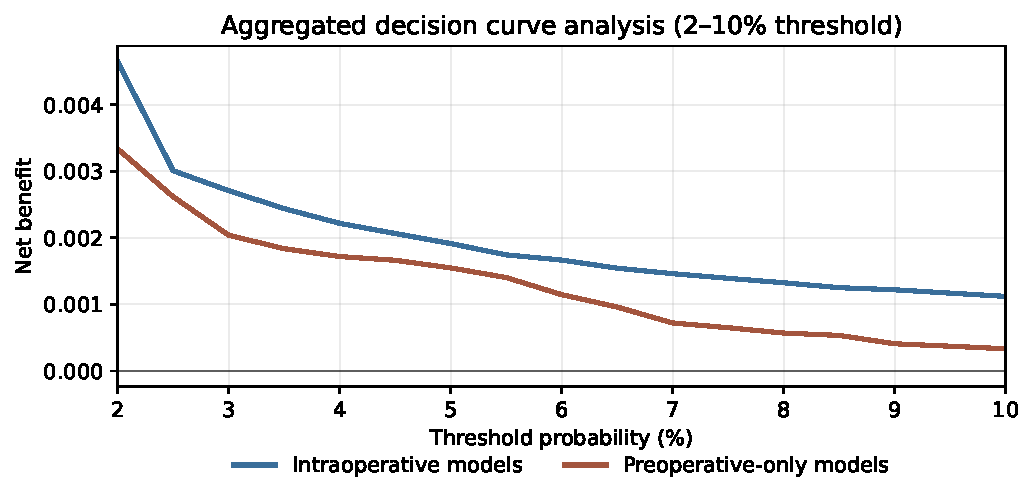
\includegraphics[width=0.85\textwidth]{figures/figure_dca_main.pdf}
\caption{Decision curve analysis at clinically relevant 2--10\%
threshold range. Mean net benefit is shown for the four
intraoperative-feature (B) models (blue) and the four preoperative-only
(A) models (brown), each averaged across the two transfer directions.
Treat-all reference is in Supplementary Figure~\ref{fig:s5-dca-detail}.
Recalibrated intraoperative models retain positive net benefit across
the \pnDcaThresholdRange\ interval; per-direction breakdown showing the
LR-INS-B utility-loss above 2\% is in Supplementary
Figure~\ref{fig:s5-dca-detail}.\\[0.5em]{\small\itshape Alt text: Decision-curve analysis plot showing mean net benefit (vertical axis) as a function of decision threshold probability (horizontal axis, 2\% to 10\%). Two curves are shown: (i) mean of the four intraoperative-feature models in blue, and (ii) mean of the four preoperative-only models in brown, each averaged across the two transfer directions (INSPIRE$\to$MOVER and MOVER$\to$INSPIRE). The intraoperative-feature curve sits above the preoperative-only curve across the entire 2--10\% threshold range, indicating that recalibrated intraoperative models retain positive net benefit for clinically realistic mortality decision thresholds. The plot's ``treat-all'' reference line (constant net benefit assuming all patients are treated) is shown in the per-direction supplementary breakdown rather than this main aggregate panel.}}
\label{fig:dca}
\end{figure}

\paragraph{Class imbalance.} Three configurations of XGB-INS-B were compared: no class weighting, the representative class weighting ($s_{pos} = 9.73$, the median per-fold tuned value from the main analysis described in \S\ref{sec:methods}), and SMOTE oversampling. Discrimination was comparable between no weighting (AUC 0.898) and the representative class weighting (AUC 0.895); SMOTE reduced external AUC by 7.7 pp (AUC 0.822), consistent with recent evidence that synthetic oversampling harms calibration and discrimination in rare-event clinical prediction~\cite{Carriero2025}.

Inferential robustness across alternative resampling configurations and three additional analyses constrained by data limitations are reported in Supplementary §S5.

% =============================================================================
